\documentclass[twoside]{book}

% Packages required by doxygen
\usepackage{fixltx2e}
\usepackage{calc}
\usepackage{doxygen}
\usepackage[export]{adjustbox} % also loads graphicx
\usepackage{graphicx}
\usepackage[utf8]{inputenc}
\usepackage{makeidx}
\usepackage{multicol}
\usepackage{multirow}
\PassOptionsToPackage{warn}{textcomp}
\usepackage{textcomp}
\usepackage[nointegrals]{wasysym}
\usepackage[table]{xcolor}

% Font selection
\usepackage[T1]{fontenc}
\usepackage[scaled=.90]{helvet}
\usepackage{courier}
\usepackage{amssymb}
\usepackage{sectsty}
\renewcommand{\familydefault}{\sfdefault}
\allsectionsfont{%
  \fontseries{bc}\selectfont%
  \color{darkgray}%
}
\renewcommand{\DoxyLabelFont}{%
  \fontseries{bc}\selectfont%
  \color{darkgray}%
}
\newcommand{\+}{\discretionary{\mbox{\scriptsize$\hookleftarrow$}}{}{}}

% Page & text layout
\usepackage{geometry}
\geometry{%
  a4paper,%
  top=2.5cm,%
  bottom=2.5cm,%
  left=2.5cm,%
  right=2.5cm%
}
\tolerance=750
\hfuzz=15pt
\hbadness=750
\setlength{\emergencystretch}{15pt}
\setlength{\parindent}{0cm}
\setlength{\parskip}{0.2cm}
\makeatletter
\renewcommand{\paragraph}{%
  \@startsection{paragraph}{4}{0ex}{-1.0ex}{1.0ex}{%
    \normalfont\normalsize\bfseries\SS@parafont%
  }%
}
\renewcommand{\subparagraph}{%
  \@startsection{subparagraph}{5}{0ex}{-1.0ex}{1.0ex}{%
    \normalfont\normalsize\bfseries\SS@subparafont%
  }%
}
\makeatother

% Headers & footers
\usepackage{fancyhdr}
\pagestyle{fancyplain}
\fancyhead[LE]{\fancyplain{}{\bfseries\thepage}}
\fancyhead[CE]{\fancyplain{}{}}
\fancyhead[RE]{\fancyplain{}{\bfseries\leftmark}}
\fancyhead[LO]{\fancyplain{}{\bfseries\rightmark}}
\fancyhead[CO]{\fancyplain{}{}}
\fancyhead[RO]{\fancyplain{}{\bfseries\thepage}}
\fancyfoot[LE]{\fancyplain{}{}}
\fancyfoot[CE]{\fancyplain{}{}}
\fancyfoot[RE]{\fancyplain{}{\bfseries\scriptsize Generated on Thu Apr 21 2016 10\+:11\+:33 for My Project by Doxygen }}
\fancyfoot[LO]{\fancyplain{}{\bfseries\scriptsize Generated on Thu Apr 21 2016 10\+:11\+:33 for My Project by Doxygen }}
\fancyfoot[CO]{\fancyplain{}{}}
\fancyfoot[RO]{\fancyplain{}{}}
\renewcommand{\footrulewidth}{0.4pt}
\renewcommand{\chaptermark}[1]{%
  \markboth{#1}{}%
}
\renewcommand{\sectionmark}[1]{%
  \markright{\thesection\ #1}%
}

% Indices & bibliography
\usepackage{natbib}
\usepackage[titles]{tocloft}
\setcounter{tocdepth}{3}
\setcounter{secnumdepth}{5}
\makeindex

% Hyperlinks (required, but should be loaded last)
\usepackage{ifpdf}
\ifpdf
  \usepackage[pdftex,pagebackref=true]{hyperref}
\else
  \usepackage[ps2pdf,pagebackref=true]{hyperref}
\fi
\hypersetup{%
  colorlinks=true,%
  linkcolor=blue,%
  citecolor=blue,%
  unicode%
}

% Custom commands
\newcommand{\clearemptydoublepage}{%
  \newpage{\pagestyle{empty}\cleardoublepage}%
}


%===== C O N T E N T S =====

\begin{document}

% Titlepage & ToC
\hypersetup{pageanchor=false,
             bookmarks=true,
             bookmarksnumbered=true,
             pdfencoding=unicode
            }
\pagenumbering{roman}
\begin{titlepage}
\vspace*{7cm}
\begin{center}%
{\Large My Project }\\
\vspace*{1cm}
{\large Generated by Doxygen 1.8.9.1}\\
\vspace*{0.5cm}
{\small Thu Apr 21 2016 10:11:33}\\
\end{center}
\end{titlepage}
\clearemptydoublepage
\tableofcontents
\clearemptydoublepage
\pagenumbering{arabic}
\hypersetup{pageanchor=true}

%--- Begin generated contents ---
\chapter{Hierarchical Index}
\section{Class Hierarchy}
This inheritance list is sorted roughly, but not completely, alphabetically\+:\begin{DoxyCompactList}
\item \contentsline{section}{tp\+:\+:Bibliographie}{\pageref{classtp_1_1Bibliographie}}{}
\item logic\+\_\+error\begin{DoxyCompactList}
\item \contentsline{section}{Contrat\+Exception}{\pageref{classContratException}}{}
\begin{DoxyCompactList}
\item \contentsline{section}{Assertion\+Exception}{\pageref{classAssertionException}}{}
\item \contentsline{section}{Invariant\+Exception}{\pageref{classInvariantException}}{}
\item \contentsline{section}{Postcondition\+Exception}{\pageref{classPostconditionException}}{}
\item \contentsline{section}{Precondition\+Exception}{\pageref{classPreconditionException}}{}
\end{DoxyCompactList}
\end{DoxyCompactList}
\item \contentsline{section}{tp\+:\+:Reference}{\pageref{classtp_1_1Reference}}{}
\begin{DoxyCompactList}
\item \contentsline{section}{tp\+:\+:Journal}{\pageref{classtp_1_1Journal}}{}
\item \contentsline{section}{tp\+:\+:Ouvrage}{\pageref{classtp_1_1Ouvrage}}{}
\end{DoxyCompactList}
\item runtime\+\_\+error\begin{DoxyCompactList}
\item \contentsline{section}{tp\+:\+:Reference\+Exception}{\pageref{classtp_1_1ReferenceException}}{}
\begin{DoxyCompactList}
\item \contentsline{section}{tp\+:\+:Reference\+Absente\+Exception}{\pageref{classtp_1_1ReferenceAbsenteException}}{}
\item \contentsline{section}{tp\+:\+:Reference\+Deja\+Presente\+Exception}{\pageref{classtp_1_1ReferenceDejaPresenteException}}{}
\end{DoxyCompactList}
\end{DoxyCompactList}
\end{DoxyCompactList}

\chapter{Class Index}
\section{Class List}
Here are the classes, structs, unions and interfaces with brief descriptions\+:\begin{DoxyCompactList}
\item\contentsline{section}{\hyperlink{classAssertionException}{Assertion\+Exception} }{\pageref{classAssertionException}}{}
\item\contentsline{section}{\hyperlink{classtp_1_1Bibliographie}{tp\+::\+Bibliographie} \\*Une classe qui permet de faire la gestion des references }{\pageref{classtp_1_1Bibliographie}}{}
\item\contentsline{section}{\hyperlink{classContratException}{Contrat\+Exception} }{\pageref{classContratException}}{}
\item\contentsline{section}{\hyperlink{classInvariantException}{Invariant\+Exception} }{\pageref{classInvariantException}}{}
\item\contentsline{section}{\hyperlink{classtp_1_1Journal}{tp\+::\+Journal} \\*Classe permettant de documenter un journal }{\pageref{classtp_1_1Journal}}{}
\item\contentsline{section}{\hyperlink{classtp_1_1Ouvrage}{tp\+::\+Ouvrage} \\*Classe permettant de documenter un \hyperlink{classtp_1_1Ouvrage}{Ouvrage} }{\pageref{classtp_1_1Ouvrage}}{}
\item\contentsline{section}{\hyperlink{classPostconditionException}{Postcondition\+Exception} }{\pageref{classPostconditionException}}{}
\item\contentsline{section}{\hyperlink{classPreconditionException}{Precondition\+Exception} }{\pageref{classPreconditionException}}{}
\item\contentsline{section}{\hyperlink{classtp_1_1Reference}{tp\+::\+Reference} \\*Classe permettant de documenter une reference }{\pageref{classtp_1_1Reference}}{}
\item\contentsline{section}{\hyperlink{classtp_1_1ReferenceAbsenteException}{tp\+::\+Reference\+Absente\+Exception} }{\pageref{classtp_1_1ReferenceAbsenteException}}{}
\item\contentsline{section}{\hyperlink{classtp_1_1ReferenceDejaPresenteException}{tp\+::\+Reference\+Deja\+Presente\+Exception} }{\pageref{classtp_1_1ReferenceDejaPresenteException}}{}
\item\contentsline{section}{\hyperlink{classtp_1_1ReferenceException}{tp\+::\+Reference\+Exception} }{\pageref{classtp_1_1ReferenceException}}{}
\end{DoxyCompactList}

\chapter{File Index}
\section{File List}
Here is a list of all documented files with brief descriptions\+:\begin{DoxyCompactList}
\item\contentsline{section}{{\bfseries Bibliographie.\+h} }{\pageref{Bibliographie_8h}}{}
\item\contentsline{section}{\hyperlink{ContratException_8cpp}{Contrat\+Exception.\+cpp} \\*Implantation de la classe \hyperlink{classContratException}{Contrat\+Exception} et de ses héritiers }{\pageref{ContratException_8cpp}}{}
\item\contentsline{section}{\hyperlink{ContratException_8h}{Contrat\+Exception.\+h} \\*D�claration de la classe \hyperlink{classContratException}{Contrat\+Exception} et de ses h�ritiers\+: std\+::logic\+\_\+error Classe de base des exceptions logiques \hyperlink{classContratException}{Contrat\+Exception}\+: Classe de base des exceptions de contrat. \hyperlink{classAssertionException}{Assertion\+Exception}\+: Classe de gestion des erreurs d\textquotesingle{}assertion. \hyperlink{classPreconditionException}{Precondition\+Exception}\+: Classe de gestion des erreurs de pr�condition. \hyperlink{classPostconditionException}{Postcondition\+Exception}\+: Classe de gestion des erreurs de postcondition. \hyperlink{classInvariantException}{Invariant\+Exception}\+: Classe de gestion des erreurs d\textquotesingle{}invariant }{\pageref{ContratException_8h}}{}
\item\contentsline{section}{{\bfseries Journal.\+h} }{\pageref{Journal_8h}}{}
\item\contentsline{section}{{\bfseries Ouvrage.\+h} }{\pageref{Ouvrage_8h}}{}
\item\contentsline{section}{{\bfseries Reference.\+h} }{\pageref{Reference_8h}}{}
\item\contentsline{section}{{\bfseries Reference\+Absente\+Exception.\+h} }{\pageref{ReferenceAbsenteException_8h}}{}
\item\contentsline{section}{{\bfseries Reference\+Deja\+Presente\+Exception.\+h} }{\pageref{ReferenceDejaPresenteException_8h}}{}
\item\contentsline{section}{{\bfseries Reference\+Exception.\+h} }{\pageref{ReferenceException_8h}}{}
\item\contentsline{section}{{\bfseries validation\+Format.\+h} }{\pageref{validationFormat_8h}}{}
\end{DoxyCompactList}

\chapter{Class Documentation}
\hypertarget{classAssertionException}{}\section{Assertion\+Exception Class Reference}
\label{classAssertionException}\index{Assertion\+Exception@{Assertion\+Exception}}


Inheritance diagram for Assertion\+Exception\+:\nopagebreak
\begin{figure}[H]
\begin{center}
\leavevmode
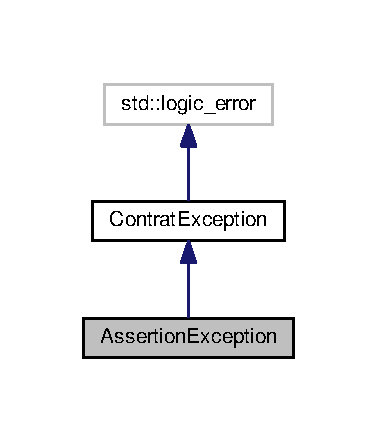
\includegraphics[width=181pt]{classAssertionException__inherit__graph}
\end{center}
\end{figure}


Collaboration diagram for Assertion\+Exception\+:\nopagebreak
\begin{figure}[H]
\begin{center}
\leavevmode
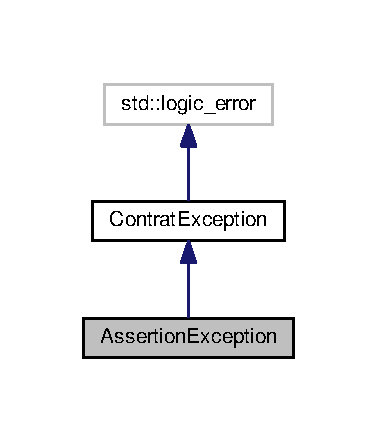
\includegraphics[width=181pt]{classAssertionException__coll__graph}
\end{center}
\end{figure}
\subsection*{Public Member Functions}
\begin{DoxyCompactItemize}
\item 
\hyperlink{classAssertionException_a93268f249b033bf4596901e50874fde6}{Assertion\+Exception} (std\+::string, unsigned int, std\+::string)
\begin{DoxyCompactList}\small\item\em Constructeur de la classe \hyperlink{classAssertionException}{Assertion\+Exception} ~\newline
 Le constructeur public \hyperlink{classAssertionException}{Assertion\+Exception}(...)initialise sa classe de base \hyperlink{classContratException}{Contrat\+Exception}. On n\textquotesingle{}a pas d\textquotesingle{}attribut local. Cette classe est intéressante pour son T\+Y\+P\+E lors du traitement des exceptions. \end{DoxyCompactList}\end{DoxyCompactItemize}


\subsection{Constructor \& Destructor Documentation}
\hypertarget{classAssertionException_a93268f249b033bf4596901e50874fde6}{}\index{Assertion\+Exception@{Assertion\+Exception}!Assertion\+Exception@{Assertion\+Exception}}
\index{Assertion\+Exception@{Assertion\+Exception}!Assertion\+Exception@{Assertion\+Exception}}
\subsubsection[{Assertion\+Exception}]{\setlength{\rightskip}{0pt plus 5cm}Assertion\+Exception\+::\+Assertion\+Exception (
\begin{DoxyParamCaption}
\item[{std\+::string}]{p\+\_\+fich\+P, }
\item[{unsigned int}]{p\+\_\+prm\+Ligne, }
\item[{std\+::string}]{p\+\_\+expr\+P}
\end{DoxyParamCaption}
)}\label{classAssertionException_a93268f249b033bf4596901e50874fde6}


Constructeur de la classe \hyperlink{classAssertionException}{Assertion\+Exception} ~\newline
 Le constructeur public \hyperlink{classAssertionException}{Assertion\+Exception}(...)initialise sa classe de base \hyperlink{classContratException}{Contrat\+Exception}. On n\textquotesingle{}a pas d\textquotesingle{}attribut local. Cette classe est intéressante pour son T\+Y\+P\+E lors du traitement des exceptions. 


\begin{DoxyParams}{Parameters}
{\em p\+\_\+fich\+P} & chaîne de caractères représentant le fichier source dans lequel a eu lieu l\textquotesingle{}erreur \\
\hline
{\em p\+\_\+prm\+Ligne} & un entier représentant la ligne où a eu lieu l\textquotesingle{}erreur \\
\hline
{\em p\+\_\+expr\+P} & Test logique qui a échoué \\
\hline
\end{DoxyParams}


The documentation for this class was generated from the following files\+:\begin{DoxyCompactItemize}
\item 
\hyperlink{ContratException_8h}{Contrat\+Exception.\+h}\item 
\hyperlink{ContratException_8cpp}{Contrat\+Exception.\+cpp}\end{DoxyCompactItemize}

\hypertarget{classtp_1_1Bibliographie}{}\section{tp\+:\+:Bibliographie Class Reference}
\label{classtp_1_1Bibliographie}\index{tp\+::\+Bibliographie@{tp\+::\+Bibliographie}}


Une classe qui permet de faire la gestion des references.  




{\ttfamily \#include $<$Bibliographie.\+h$>$}

\subsection*{Public Member Functions}
\begin{DoxyCompactItemize}
\item 
\hypertarget{classtp_1_1Bibliographie_a421ef2a88d9bebe630723aef9715fcda}{}\hyperlink{classtp_1_1Bibliographie_a421ef2a88d9bebe630723aef9715fcda}{Bibliographie} ()\label{classtp_1_1Bibliographie_a421ef2a88d9bebe630723aef9715fcda}

\begin{DoxyCompactList}\small\item\em Constructeur sans paramètres. \end{DoxyCompactList}\item 
\hypertarget{classtp_1_1Bibliographie_a6b304f77486829238679d517ec0d5389}{}virtual \hyperlink{classtp_1_1Bibliographie_a6b304f77486829238679d517ec0d5389}{$\sim$\+Bibliographie} ()\label{classtp_1_1Bibliographie_a6b304f77486829238679d517ec0d5389}

\begin{DoxyCompactList}\small\item\em Destructeur de la classe \hyperlink{classtp_1_1Bibliographie}{Bibliographie}. \end{DoxyCompactList}\item 
\hypertarget{classtp_1_1Bibliographie_ac4650643e18de38f4d95e4fbff7614ea}{}void \hyperlink{classtp_1_1Bibliographie_ac4650643e18de38f4d95e4fbff7614ea}{ajouter\+Reference} (const \hyperlink{classtp_1_1Reference}{Reference} \&p\+\_\+\+Reference)\label{classtp_1_1Bibliographie_ac4650643e18de38f4d95e4fbff7614ea}

\begin{DoxyCompactList}\small\item\em Méthode pour ajouter une référence au vecteur des références. \end{DoxyCompactList}\item 
\hypertarget{classtp_1_1Bibliographie_a5a3fc571e6c6dfe1934f766ef5a7fda8}{}void \hyperlink{classtp_1_1Bibliographie_a5a3fc571e6c6dfe1934f766ef5a7fda8}{supprimer\+Reference} (const std\+::string \&p\+\_\+identifiant)\label{classtp_1_1Bibliographie_a5a3fc571e6c6dfe1934f766ef5a7fda8}

\begin{DoxyCompactList}\small\item\em Méthode pour supprimer une reference dans la bibliographie. \end{DoxyCompactList}\item 
\hypertarget{classtp_1_1Bibliographie_adf99092c98d0360e886b0645544a699d}{}unsigned \hyperlink{classtp_1_1Bibliographie_adf99092c98d0360e886b0645544a699d}{nb\+References} () const \label{classtp_1_1Bibliographie_adf99092c98d0360e886b0645544a699d}

\begin{DoxyCompactList}\small\item\em Méthode pour avoir le nombre de references dans la bibliographie. \end{DoxyCompactList}\item 
std\+::string \hyperlink{classtp_1_1Bibliographie_a8740e1fd550e455b5846945d54f308b4}{req\+Bibliographie\+Formate} () const 
\begin{DoxyCompactList}\small\item\em Retourne une chaine de caractere qui contient l\textquotesingle{}information de l\textquotesingle{}objet \hyperlink{classtp_1_1Bibliographie}{Bibliographie}. \end{DoxyCompactList}\end{DoxyCompactItemize}


\subsection{Detailed Description}
Une classe qui permet de faire la gestion des references. 

\subsection{Member Function Documentation}
\hypertarget{classtp_1_1Bibliographie_a8740e1fd550e455b5846945d54f308b4}{}\index{tp\+::\+Bibliographie@{tp\+::\+Bibliographie}!req\+Bibliographie\+Formate@{req\+Bibliographie\+Formate}}
\index{req\+Bibliographie\+Formate@{req\+Bibliographie\+Formate}!tp\+::\+Bibliographie@{tp\+::\+Bibliographie}}
\subsubsection[{req\+Bibliographie\+Formate}]{\setlength{\rightskip}{0pt plus 5cm}std\+::string tp\+::\+Bibliographie\+::req\+Bibliographie\+Formate (
\begin{DoxyParamCaption}
{}
\end{DoxyParamCaption}
) const}\label{classtp_1_1Bibliographie_a8740e1fd550e455b5846945d54f308b4}


Retourne une chaine de caractere qui contient l\textquotesingle{}information de l\textquotesingle{}objet \hyperlink{classtp_1_1Bibliographie}{Bibliographie}. 

\begin{DoxyReturn}{Returns}
un string qui contient l\textquotesingle{}information 
\end{DoxyReturn}


The documentation for this class was generated from the following files\+:\begin{DoxyCompactItemize}
\item 
Bibliographie.\+h\item 
Bibliographie.\+cpp\end{DoxyCompactItemize}

\hypertarget{classContratException}{}\section{Contrat\+Exception Class Reference}
\label{classContratException}\index{Contrat\+Exception@{Contrat\+Exception}}


Inheritance diagram for Contrat\+Exception\+:\nopagebreak
\begin{figure}[H]
\begin{center}
\leavevmode
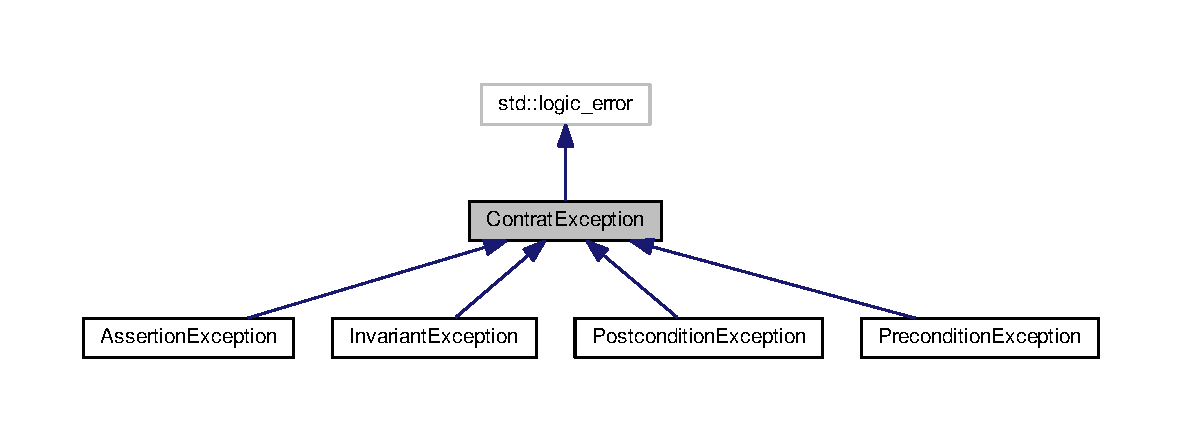
\includegraphics[width=350pt]{classContratException__inherit__graph}
\end{center}
\end{figure}


Collaboration diagram for Contrat\+Exception\+:\nopagebreak
\begin{figure}[H]
\begin{center}
\leavevmode
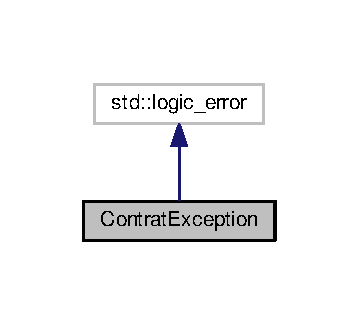
\includegraphics[width=172pt]{classContratException__coll__graph}
\end{center}
\end{figure}
\subsection*{Public Member Functions}
\begin{DoxyCompactItemize}
\item 
\hyperlink{classContratException_ad6c04fb577e960f87e010b125aa636a0}{Contrat\+Exception} (std\+::string, unsigned int, std\+::string, std\+::string)
\begin{DoxyCompactList}\small\item\em Constructeur de la classe de base \hyperlink{classContratException}{Contrat\+Exception}. \end{DoxyCompactList}\item 
std\+::string \hyperlink{classContratException_a8d20a9959f3b7cc4334165794dbaf1fc}{req\+Texte\+Exception} () const 
\begin{DoxyCompactList}\small\item\em Construit le texte complet relié à l\textquotesingle{}exception de contrat. \end{DoxyCompactList}\end{DoxyCompactItemize}


\subsection{Constructor \& Destructor Documentation}
\hypertarget{classContratException_ad6c04fb577e960f87e010b125aa636a0}{}\index{Contrat\+Exception@{Contrat\+Exception}!Contrat\+Exception@{Contrat\+Exception}}
\index{Contrat\+Exception@{Contrat\+Exception}!Contrat\+Exception@{Contrat\+Exception}}
\subsubsection[{Contrat\+Exception}]{\setlength{\rightskip}{0pt plus 5cm}Contrat\+Exception\+::\+Contrat\+Exception (
\begin{DoxyParamCaption}
\item[{std\+::string}]{p\+\_\+fich\+P, }
\item[{unsigned int}]{p\+\_\+prm\+Ligne, }
\item[{std\+::string}]{p\+\_\+expr\+P, }
\item[{std\+::string}]{p\+\_\+msg\+P}
\end{DoxyParamCaption}
)}\label{classContratException_ad6c04fb577e960f87e010b125aa636a0}


Constructeur de la classe de base \hyperlink{classContratException}{Contrat\+Exception}. 


\begin{DoxyParams}{Parameters}
{\em p\+\_\+fich\+P} & chaîne de caractères représentant le fichier source dans lequel a eu lieu l\textquotesingle{}erreur \\
\hline
{\em p\+\_\+prm\+Ligne} & un entier représentant la ligne où a eu lieu l\textquotesingle{}erreur \\
\hline
{\em p\+\_\+msg\+P} & Message décrivant l\textquotesingle{}erreur \\
\hline
{\em p\+\_\+expr\+P} & Test logique qui a échoué \\
\hline
\end{DoxyParams}


\subsection{Member Function Documentation}
\hypertarget{classContratException_a8d20a9959f3b7cc4334165794dbaf1fc}{}\index{Contrat\+Exception@{Contrat\+Exception}!req\+Texte\+Exception@{req\+Texte\+Exception}}
\index{req\+Texte\+Exception@{req\+Texte\+Exception}!Contrat\+Exception@{Contrat\+Exception}}
\subsubsection[{req\+Texte\+Exception}]{\setlength{\rightskip}{0pt plus 5cm}std\+::string Contrat\+Exception\+::req\+Texte\+Exception (
\begin{DoxyParamCaption}
{}
\end{DoxyParamCaption}
) const}\label{classContratException_a8d20a9959f3b7cc4334165794dbaf1fc}


Construit le texte complet relié à l\textquotesingle{}exception de contrat. 

\begin{DoxyReturn}{Returns}
une chaîne de caractères correspondant à l\textquotesingle{}exception 
\end{DoxyReturn}


The documentation for this class was generated from the following files\+:\begin{DoxyCompactItemize}
\item 
\hyperlink{ContratException_8h}{Contrat\+Exception.\+h}\item 
\hyperlink{ContratException_8cpp}{Contrat\+Exception.\+cpp}\end{DoxyCompactItemize}

\hypertarget{classInvariantException}{}\section{Invariant\+Exception Class Reference}
\label{classInvariantException}\index{Invariant\+Exception@{Invariant\+Exception}}


Inheritance diagram for Invariant\+Exception\+:\nopagebreak
\begin{figure}[H]
\begin{center}
\leavevmode
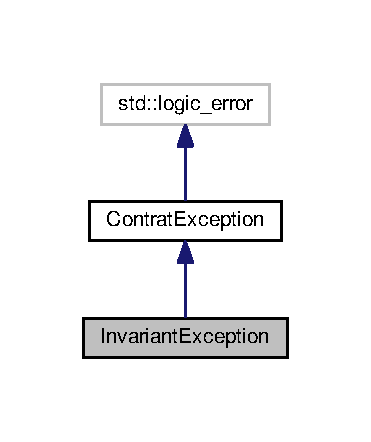
\includegraphics[width=178pt]{classInvariantException__inherit__graph}
\end{center}
\end{figure}


Collaboration diagram for Invariant\+Exception\+:\nopagebreak
\begin{figure}[H]
\begin{center}
\leavevmode
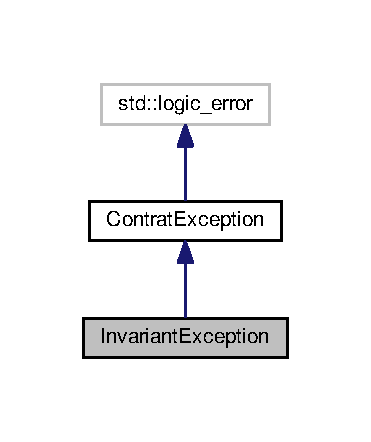
\includegraphics[width=178pt]{classInvariantException__coll__graph}
\end{center}
\end{figure}
\subsection*{Public Member Functions}
\begin{DoxyCompactItemize}
\item 
\hyperlink{classInvariantException_af8a1950834b26c256db0b11eb33e6056}{Invariant\+Exception} (std\+::string, unsigned int, std\+::string)
\begin{DoxyCompactList}\small\item\em Constructeur de la classe \hyperlink{classInvariantException}{Invariant\+Exception} en initialisant la classe de base \hyperlink{classContratException}{Contrat\+Exception}. La classe représente des erreurs d\textquotesingle{}invariant dans la théorie du contrat. \end{DoxyCompactList}\end{DoxyCompactItemize}


\subsection{Constructor \& Destructor Documentation}
\hypertarget{classInvariantException_af8a1950834b26c256db0b11eb33e6056}{}\index{Invariant\+Exception@{Invariant\+Exception}!Invariant\+Exception@{Invariant\+Exception}}
\index{Invariant\+Exception@{Invariant\+Exception}!Invariant\+Exception@{Invariant\+Exception}}
\subsubsection[{Invariant\+Exception}]{\setlength{\rightskip}{0pt plus 5cm}Invariant\+Exception\+::\+Invariant\+Exception (
\begin{DoxyParamCaption}
\item[{std\+::string}]{p\+\_\+fich\+P, }
\item[{unsigned int}]{p\+\_\+prm\+Ligne, }
\item[{std\+::string}]{p\+\_\+expr\+P}
\end{DoxyParamCaption}
)}\label{classInvariantException_af8a1950834b26c256db0b11eb33e6056}


Constructeur de la classe \hyperlink{classInvariantException}{Invariant\+Exception} en initialisant la classe de base \hyperlink{classContratException}{Contrat\+Exception}. La classe représente des erreurs d\textquotesingle{}invariant dans la théorie du contrat. 


\begin{DoxyParams}{Parameters}
{\em p\+\_\+fich\+P} & chaîne de caractères représentant le fichier source dans lequel a eu lieu l\textquotesingle{}erreur \\
\hline
{\em p\+\_\+prm\+Ligne} & un entier représentant la ligne où a eu lieu l\textquotesingle{}erreur \\
\hline
{\em p\+\_\+expr\+P} & Test logique qui a échoué \\
\hline
\end{DoxyParams}


The documentation for this class was generated from the following files\+:\begin{DoxyCompactItemize}
\item 
\hyperlink{ContratException_8h}{Contrat\+Exception.\+h}\item 
\hyperlink{ContratException_8cpp}{Contrat\+Exception.\+cpp}\end{DoxyCompactItemize}

\hypertarget{classtp_1_1Journal}{}\section{tp\+:\+:Journal Class Reference}
\label{classtp_1_1Journal}\index{tp\+::\+Journal@{tp\+::\+Journal}}


Classe permettant de documenter un journal.  




{\ttfamily \#include $<$Journal.\+h$>$}



Inheritance diagram for tp\+:\+:Journal\+:\nopagebreak
\begin{figure}[H]
\begin{center}
\leavevmode
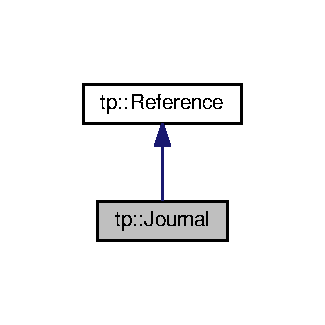
\includegraphics[width=156pt]{classtp_1_1Journal__inherit__graph}
\end{center}
\end{figure}


Collaboration diagram for tp\+:\+:Journal\+:\nopagebreak
\begin{figure}[H]
\begin{center}
\leavevmode
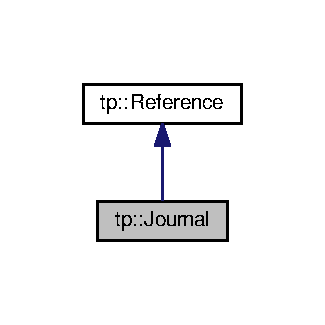
\includegraphics[width=156pt]{classtp_1_1Journal__coll__graph}
\end{center}
\end{figure}
\subsection*{Public Member Functions}
\begin{DoxyCompactItemize}
\item 
\hyperlink{classtp_1_1Journal_a29ba681f3e9c3c755f0903de6163b04a}{Journal} (const std\+::string \&p\+\_\+auteurs, const std\+::string \&p\+\_\+titre, const std\+::string \&p\+\_\+identifiant, unsigned p\+\_\+annee, const std\+::string \&p\+\_\+nom, unsigned p\+\_\+volume, unsigned p\+\_\+numero, unsigned p\+\_\+page)
\begin{DoxyCompactList}\small\item\em Constructeur de la classe \hyperlink{classtp_1_1Journal}{Journal} Les parametres de cette classe sont\+: \end{DoxyCompactList}\item 
const std\+::string \& \hyperlink{classtp_1_1Journal_a86f42ccad53aba8a6751e22f93e31e0b}{req\+Nom} () const 
\item 
unsigned \hyperlink{classtp_1_1Journal_aded8daafc9b7825d25c66191b14ac837}{req\+Volume} () const 
\item 
unsigned \hyperlink{classtp_1_1Journal_ac4a5da3c7d51cac23f661ff57daa49aa}{req\+Numero} () const 
\item 
unsigned \hyperlink{classtp_1_1Journal_a769fa7159eacd6afffd2ce704a38c370}{req\+Page} () const 
\item 
\hypertarget{classtp_1_1Journal_a4a2c3775789f5db43e4fc7312ef9624a}{}void \hyperlink{classtp_1_1Journal_a4a2c3775789f5db43e4fc7312ef9624a}{asg\+Nom} (const std\+::string \&p\+\_\+nom)\label{classtp_1_1Journal_a4a2c3775789f5db43e4fc7312ef9624a}

\begin{DoxyCompactList}\small\item\em Mutateur pour nom, modifie le nom. \end{DoxyCompactList}\item 
\hypertarget{classtp_1_1Journal_a9aa261a1fc5aa170127042e88e281115}{}void \hyperlink{classtp_1_1Journal_a9aa261a1fc5aa170127042e88e281115}{asg\+Volume} (unsigned p\+\_\+volume)\label{classtp_1_1Journal_a9aa261a1fc5aa170127042e88e281115}

\begin{DoxyCompactList}\small\item\em Mutateur pour volume, modifie le volume. \end{DoxyCompactList}\item 
\hypertarget{classtp_1_1Journal_aa1a08e16b6eb8482e5f2dc40af471b24}{}void \hyperlink{classtp_1_1Journal_aa1a08e16b6eb8482e5f2dc40af471b24}{asg\+Numero} (unsigned p\+\_\+numero)\label{classtp_1_1Journal_aa1a08e16b6eb8482e5f2dc40af471b24}

\begin{DoxyCompactList}\small\item\em Mutateur pour numero, modifie le numero. \end{DoxyCompactList}\item 
\hypertarget{classtp_1_1Journal_a70c16c8d5211258396c801de34705ef6}{}void \hyperlink{classtp_1_1Journal_a70c16c8d5211258396c801de34705ef6}{asg\+Page} (unsigned p\+\_\+page)\label{classtp_1_1Journal_a70c16c8d5211258396c801de34705ef6}

\begin{DoxyCompactList}\small\item\em Mutateur pour page, modifie la page. \end{DoxyCompactList}\item 
virtual std\+::string \hyperlink{classtp_1_1Journal_adbc714005b9d394b6b76ba7f5f9f560f}{req\+Reference\+Formate} () const 
\item 
\hypertarget{classtp_1_1Journal_ade5cb6f330a331f626f27b877617a723}{}virtual \hyperlink{classtp_1_1Reference}{Reference} $\ast$ {\bfseries clone} () const \label{classtp_1_1Journal_ade5cb6f330a331f626f27b877617a723}

\item 
\hypertarget{classtp_1_1Journal_a532b58f942cbaf5fce074e5ca7a5ee54}{}void {\bfseries verifie\+Invariant} () const \label{classtp_1_1Journal_a532b58f942cbaf5fce074e5ca7a5ee54}

\end{DoxyCompactItemize}
\subsection*{Public Attributes}
\begin{DoxyCompactItemize}
\item 
\hypertarget{classtp_1_1Journal_a887da7c6effea08f87f9f2769fd55ac9}{}std\+::string {\bfseries m\+\_\+nom}\label{classtp_1_1Journal_a887da7c6effea08f87f9f2769fd55ac9}

\item 
\hypertarget{classtp_1_1Journal_a86783fee0013f17545b9563b9bfa69ec}{}unsigned {\bfseries m\+\_\+volume}\label{classtp_1_1Journal_a86783fee0013f17545b9563b9bfa69ec}

\item 
\hypertarget{classtp_1_1Journal_aaa4bbd5bed61481d0085472bca39ddc2}{}unsigned {\bfseries m\+\_\+numero}\label{classtp_1_1Journal_aaa4bbd5bed61481d0085472bca39ddc2}

\item 
\hypertarget{classtp_1_1Journal_a4d4d2155cec44c454848c47fe4001393}{}unsigned {\bfseries m\+\_\+page}\label{classtp_1_1Journal_a4d4d2155cec44c454848c47fe4001393}

\end{DoxyCompactItemize}


\subsection{Detailed Description}
Classe permettant de documenter un journal. 

de la classe derivée \hyperlink{classtp_1_1Journal}{Journal} 

\subsection{Constructor \& Destructor Documentation}
\hypertarget{classtp_1_1Journal_a29ba681f3e9c3c755f0903de6163b04a}{}\index{tp\+::\+Journal@{tp\+::\+Journal}!Journal@{Journal}}
\index{Journal@{Journal}!tp\+::\+Journal@{tp\+::\+Journal}}
\subsubsection[{Journal}]{\setlength{\rightskip}{0pt plus 5cm}tp\+::\+Journal\+::\+Journal (
\begin{DoxyParamCaption}
\item[{const std\+::string \&}]{p\+\_\+auteurs, }
\item[{const std\+::string \&}]{p\+\_\+titre, }
\item[{const std\+::string \&}]{p\+\_\+identifiant, }
\item[{unsigned}]{p\+\_\+annee, }
\item[{const std\+::string \&}]{p\+\_\+nom, }
\item[{unsigned}]{p\+\_\+volume, }
\item[{unsigned}]{p\+\_\+numero, }
\item[{unsigned}]{p\+\_\+page}
\end{DoxyParamCaption}
)}\label{classtp_1_1Journal_a29ba681f3e9c3c755f0903de6163b04a}


Constructeur de la classe \hyperlink{classtp_1_1Journal}{Journal} Les parametres de cette classe sont\+: 


\begin{DoxyParams}{Parameters}
{\em p\+\_\+auteurs} & du journal \\
\hline
{\em p\+\_\+titre} & du journal \\
\hline
{\em p\+\_\+identifiant} & (Code I\+S\+B\+N) du journal \\
\hline
{\em p\+\_\+annee} & du journal \\
\hline
{\em p\+\_\+nom} & du journal \\
\hline
{\em p\+\_\+volume} & du journal \\
\hline
{\em p\+\_\+nuemro} & du journal \\
\hline
{\em p\+\_\+page} & du journal \\
\hline
\end{DoxyParams}


\subsection{Member Function Documentation}
\hypertarget{classtp_1_1Journal_a86f42ccad53aba8a6751e22f93e31e0b}{}\index{tp\+::\+Journal@{tp\+::\+Journal}!req\+Nom@{req\+Nom}}
\index{req\+Nom@{req\+Nom}!tp\+::\+Journal@{tp\+::\+Journal}}
\subsubsection[{req\+Nom}]{\setlength{\rightskip}{0pt plus 5cm}const std\+::string \& tp\+::\+Journal\+::req\+Nom (
\begin{DoxyParamCaption}
{}
\end{DoxyParamCaption}
) const}\label{classtp_1_1Journal_a86f42ccad53aba8a6751e22f93e31e0b}
brief Acceseur pour req\+Nom return m\+\_\+nom le nom de l\textquotesingle{}objet \hypertarget{classtp_1_1Journal_ac4a5da3c7d51cac23f661ff57daa49aa}{}\index{tp\+::\+Journal@{tp\+::\+Journal}!req\+Numero@{req\+Numero}}
\index{req\+Numero@{req\+Numero}!tp\+::\+Journal@{tp\+::\+Journal}}
\subsubsection[{req\+Numero}]{\setlength{\rightskip}{0pt plus 5cm}unsigned tp\+::\+Journal\+::req\+Numero (
\begin{DoxyParamCaption}
{}
\end{DoxyParamCaption}
) const}\label{classtp_1_1Journal_ac4a5da3c7d51cac23f661ff57daa49aa}
brief Acceseur pour req\+Numero return m\+\_\+numero le numero de l\textquotesingle{}objet \hypertarget{classtp_1_1Journal_a769fa7159eacd6afffd2ce704a38c370}{}\index{tp\+::\+Journal@{tp\+::\+Journal}!req\+Page@{req\+Page}}
\index{req\+Page@{req\+Page}!tp\+::\+Journal@{tp\+::\+Journal}}
\subsubsection[{req\+Page}]{\setlength{\rightskip}{0pt plus 5cm}unsigned tp\+::\+Journal\+::req\+Page (
\begin{DoxyParamCaption}
{}
\end{DoxyParamCaption}
) const}\label{classtp_1_1Journal_a769fa7159eacd6afffd2ce704a38c370}
brief Acceseur pour req\+Page return m\+\_\+page la page de l\textquotesingle{}objet \hypertarget{classtp_1_1Journal_adbc714005b9d394b6b76ba7f5f9f560f}{}\index{tp\+::\+Journal@{tp\+::\+Journal}!req\+Reference\+Formate@{req\+Reference\+Formate}}
\index{req\+Reference\+Formate@{req\+Reference\+Formate}!tp\+::\+Journal@{tp\+::\+Journal}}
\subsubsection[{req\+Reference\+Formate}]{\setlength{\rightskip}{0pt plus 5cm}std\+::string tp\+::\+Journal\+::req\+Reference\+Formate (
\begin{DoxyParamCaption}
{}
\end{DoxyParamCaption}
) const\hspace{0.3cm}{\ttfamily [virtual]}}\label{classtp_1_1Journal_adbc714005b9d394b6b76ba7f5f9f560f}
brief Acceseur pour pour req\+Reference\+Formate return le format des références 

Implements \hyperlink{classtp_1_1Reference_af166101d908f6d0f8edeb8624aa77a9b}{tp\+::\+Reference}.

\hypertarget{classtp_1_1Journal_aded8daafc9b7825d25c66191b14ac837}{}\index{tp\+::\+Journal@{tp\+::\+Journal}!req\+Volume@{req\+Volume}}
\index{req\+Volume@{req\+Volume}!tp\+::\+Journal@{tp\+::\+Journal}}
\subsubsection[{req\+Volume}]{\setlength{\rightskip}{0pt plus 5cm}unsigned tp\+::\+Journal\+::req\+Volume (
\begin{DoxyParamCaption}
{}
\end{DoxyParamCaption}
) const}\label{classtp_1_1Journal_aded8daafc9b7825d25c66191b14ac837}
brief Acceseur pour req\+Volume return m\+\_\+volume le volume de l\textquotesingle{}objet 

The documentation for this class was generated from the following files\+:\begin{DoxyCompactItemize}
\item 
Journal.\+h\item 
Journal.\+cpp\end{DoxyCompactItemize}

\hypertarget{classtp_1_1Ouvrage}{}\section{tp\+:\+:Ouvrage Class Reference}
\label{classtp_1_1Ouvrage}\index{tp\+::\+Ouvrage@{tp\+::\+Ouvrage}}


Classe permettant de documenter un \hyperlink{classtp_1_1Ouvrage}{Ouvrage}.  




{\ttfamily \#include $<$Ouvrage.\+h$>$}



Inheritance diagram for tp\+:\+:Ouvrage\+:\nopagebreak
\begin{figure}[H]
\begin{center}
\leavevmode
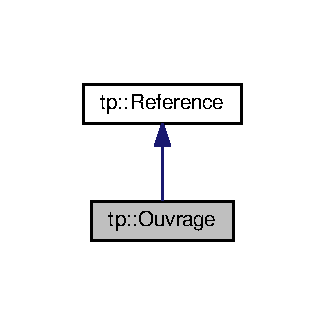
\includegraphics[width=156pt]{classtp_1_1Ouvrage__inherit__graph}
\end{center}
\end{figure}


Collaboration diagram for tp\+:\+:Ouvrage\+:\nopagebreak
\begin{figure}[H]
\begin{center}
\leavevmode
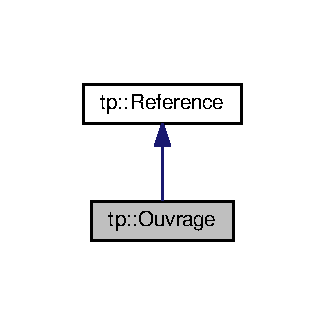
\includegraphics[width=156pt]{classtp_1_1Ouvrage__coll__graph}
\end{center}
\end{figure}
\subsection*{Public Member Functions}
\begin{DoxyCompactItemize}
\item 
\hyperlink{classtp_1_1Ouvrage_a32d83af26a17b517d3188cca4c443b5e}{Ouvrage} (const std\+::string \&p\+\_\+auteurs, const std\+::string \&p\+\_\+titre, const std\+::string \&p\+\_\+identifiant, unsigned p\+\_\+annee, const std\+::string \&p\+\_\+ville, const std\+::string \&p\+\_\+editeur)
\begin{DoxyCompactList}\small\item\em Constructeur de la classe \hyperlink{classtp_1_1Ouvrage}{Ouvrage} Les parametres de cette classe sont\+: \end{DoxyCompactList}\item 
const std\+::string \& \hyperlink{classtp_1_1Ouvrage_aa25d4d5050ac2650a6a502b57b95f786}{req\+Ville} () const 
\item 
const std\+::string \& \hyperlink{classtp_1_1Ouvrage_a43319c7254bd4dec49437d1c78b914d0}{req\+Editeur} () const 
\item 
\hypertarget{classtp_1_1Ouvrage_a2547ac0a613d7583c06b4cc13f8abd9a}{}void \hyperlink{classtp_1_1Ouvrage_a2547ac0a613d7583c06b4cc13f8abd9a}{asg\+Ville} (const std\+::string \&p\+\_\+ville)\label{classtp_1_1Ouvrage_a2547ac0a613d7583c06b4cc13f8abd9a}

\begin{DoxyCompactList}\small\item\em Mutateur pour ville, modifie la ville. \end{DoxyCompactList}\item 
\hypertarget{classtp_1_1Ouvrage_a6a3762a00735d48498f1e406057a7678}{}void \hyperlink{classtp_1_1Ouvrage_a6a3762a00735d48498f1e406057a7678}{asg\+Editeur} (const std\+::string \&p\+\_\+editeur)\label{classtp_1_1Ouvrage_a6a3762a00735d48498f1e406057a7678}

\begin{DoxyCompactList}\small\item\em Mutateur pour editeur, modifie l\textquotesingle{}editeur. \end{DoxyCompactList}\item 
virtual std\+::string \hyperlink{classtp_1_1Ouvrage_a72a27ae3d11d41e3f02021c671e9a50a}{req\+Reference\+Formate} () const 
\item 
\hypertarget{classtp_1_1Ouvrage_a8e50d795c1e7d5b99dea1357e4282e12}{}virtual \hyperlink{classtp_1_1Reference}{Reference} $\ast$ {\bfseries clone} () const \label{classtp_1_1Ouvrage_a8e50d795c1e7d5b99dea1357e4282e12}

\end{DoxyCompactItemize}


\subsection{Detailed Description}
Classe permettant de documenter un \hyperlink{classtp_1_1Ouvrage}{Ouvrage}. 

de la classe derivée \hyperlink{classtp_1_1Ouvrage}{Ouvrage} 

\subsection{Constructor \& Destructor Documentation}
\hypertarget{classtp_1_1Ouvrage_a32d83af26a17b517d3188cca4c443b5e}{}\index{tp\+::\+Ouvrage@{tp\+::\+Ouvrage}!Ouvrage@{Ouvrage}}
\index{Ouvrage@{Ouvrage}!tp\+::\+Ouvrage@{tp\+::\+Ouvrage}}
\subsubsection[{Ouvrage}]{\setlength{\rightskip}{0pt plus 5cm}tp\+::\+Ouvrage\+::\+Ouvrage (
\begin{DoxyParamCaption}
\item[{const std\+::string \&}]{p\+\_\+auteurs, }
\item[{const std\+::string \&}]{p\+\_\+titre, }
\item[{const std\+::string \&}]{p\+\_\+identifiant, }
\item[{unsigned}]{p\+\_\+annee, }
\item[{const std\+::string \&}]{p\+\_\+ville, }
\item[{const std\+::string \&}]{p\+\_\+editeur}
\end{DoxyParamCaption}
)}\label{classtp_1_1Ouvrage_a32d83af26a17b517d3188cca4c443b5e}


Constructeur de la classe \hyperlink{classtp_1_1Ouvrage}{Ouvrage} Les parametres de cette classe sont\+: 


\begin{DoxyParams}{Parameters}
{\em p\+\_\+auteurs} & de l\textquotesingle{}ouvrage \\
\hline
{\em p\+\_\+titre} & de l\textquotesingle{}ouvrage \\
\hline
{\em p\+\_\+identifiant} & (Code I\+S\+B\+N) de l\textquotesingle{}ouvrage \\
\hline
{\em p\+\_\+annee} & de l\textquotesingle{}ouvrage \\
\hline
{\em p\+\_\+ville} & de l\textquotesingle{}ouvrage \\
\hline
{\em p\+\_\+editeur} & de l\textquotesingle{}ouvrage \\
\hline
\end{DoxyParams}


\subsection{Member Function Documentation}
\hypertarget{classtp_1_1Ouvrage_a43319c7254bd4dec49437d1c78b914d0}{}\index{tp\+::\+Ouvrage@{tp\+::\+Ouvrage}!req\+Editeur@{req\+Editeur}}
\index{req\+Editeur@{req\+Editeur}!tp\+::\+Ouvrage@{tp\+::\+Ouvrage}}
\subsubsection[{req\+Editeur}]{\setlength{\rightskip}{0pt plus 5cm}const std\+::string \& tp\+::\+Ouvrage\+::req\+Editeur (
\begin{DoxyParamCaption}
{}
\end{DoxyParamCaption}
) const}\label{classtp_1_1Ouvrage_a43319c7254bd4dec49437d1c78b914d0}
brief Acceseur pour req\+Editeur return m\+\_\+editeur l\textquotesingle{}editeur de l\textquotesingle{}objet \hypertarget{classtp_1_1Ouvrage_a72a27ae3d11d41e3f02021c671e9a50a}{}\index{tp\+::\+Ouvrage@{tp\+::\+Ouvrage}!req\+Reference\+Formate@{req\+Reference\+Formate}}
\index{req\+Reference\+Formate@{req\+Reference\+Formate}!tp\+::\+Ouvrage@{tp\+::\+Ouvrage}}
\subsubsection[{req\+Reference\+Formate}]{\setlength{\rightskip}{0pt plus 5cm}std\+::string tp\+::\+Ouvrage\+::req\+Reference\+Formate (
\begin{DoxyParamCaption}
{}
\end{DoxyParamCaption}
) const\hspace{0.3cm}{\ttfamily [virtual]}}\label{classtp_1_1Ouvrage_a72a27ae3d11d41e3f02021c671e9a50a}
brief Acceseur pour pour req\+Reference\+Formate return le format des références 

Implements \hyperlink{classtp_1_1Reference_af166101d908f6d0f8edeb8624aa77a9b}{tp\+::\+Reference}.

\hypertarget{classtp_1_1Ouvrage_aa25d4d5050ac2650a6a502b57b95f786}{}\index{tp\+::\+Ouvrage@{tp\+::\+Ouvrage}!req\+Ville@{req\+Ville}}
\index{req\+Ville@{req\+Ville}!tp\+::\+Ouvrage@{tp\+::\+Ouvrage}}
\subsubsection[{req\+Ville}]{\setlength{\rightskip}{0pt plus 5cm}const std\+::string \& tp\+::\+Ouvrage\+::req\+Ville (
\begin{DoxyParamCaption}
{}
\end{DoxyParamCaption}
) const}\label{classtp_1_1Ouvrage_aa25d4d5050ac2650a6a502b57b95f786}
brief Acceseur pour req\+Ville return m\+\_\+ville la ville de l\textquotesingle{}objet 

The documentation for this class was generated from the following files\+:\begin{DoxyCompactItemize}
\item 
Ouvrage.\+h\item 
Ouvrage.\+cpp\end{DoxyCompactItemize}

\hypertarget{classPostconditionException}{}\section{Postcondition\+Exception Class Reference}
\label{classPostconditionException}\index{Postcondition\+Exception@{Postcondition\+Exception}}


Inheritance diagram for Postcondition\+Exception\+:\nopagebreak
\begin{figure}[H]
\begin{center}
\leavevmode
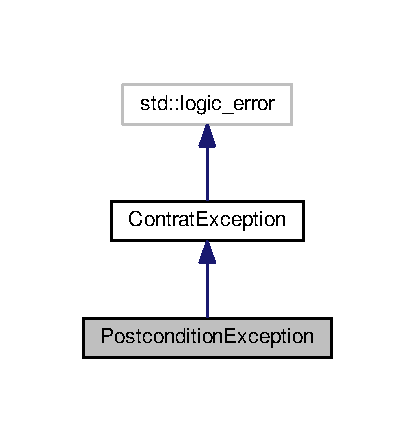
\includegraphics[width=199pt]{classPostconditionException__inherit__graph}
\end{center}
\end{figure}


Collaboration diagram for Postcondition\+Exception\+:\nopagebreak
\begin{figure}[H]
\begin{center}
\leavevmode
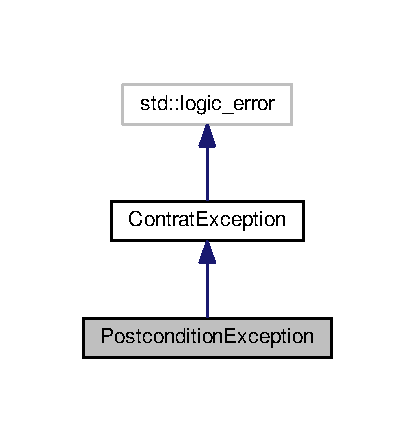
\includegraphics[width=199pt]{classPostconditionException__coll__graph}
\end{center}
\end{figure}
\subsection*{Public Member Functions}
\begin{DoxyCompactItemize}
\item 
\hyperlink{classPostconditionException_acc95ea17c4302b996261b7201d2cf6c4}{Postcondition\+Exception} (std\+::string, unsigned int, std\+::string)
\begin{DoxyCompactList}\small\item\em Constructeur de la classe \hyperlink{classPostconditionException}{Postcondition\+Exception} en initialisant la classe de base \hyperlink{classContratException}{Contrat\+Exception}. La classe représente des erreurs de postcondition dans la théorie du contrat. \end{DoxyCompactList}\end{DoxyCompactItemize}


\subsection{Constructor \& Destructor Documentation}
\hypertarget{classPostconditionException_acc95ea17c4302b996261b7201d2cf6c4}{}\index{Postcondition\+Exception@{Postcondition\+Exception}!Postcondition\+Exception@{Postcondition\+Exception}}
\index{Postcondition\+Exception@{Postcondition\+Exception}!Postcondition\+Exception@{Postcondition\+Exception}}
\subsubsection[{Postcondition\+Exception}]{\setlength{\rightskip}{0pt plus 5cm}Postcondition\+Exception\+::\+Postcondition\+Exception (
\begin{DoxyParamCaption}
\item[{std\+::string}]{p\+\_\+fich\+P, }
\item[{unsigned int}]{p\+\_\+prm\+Ligne, }
\item[{std\+::string}]{p\+\_\+expr\+P}
\end{DoxyParamCaption}
)}\label{classPostconditionException_acc95ea17c4302b996261b7201d2cf6c4}


Constructeur de la classe \hyperlink{classPostconditionException}{Postcondition\+Exception} en initialisant la classe de base \hyperlink{classContratException}{Contrat\+Exception}. La classe représente des erreurs de postcondition dans la théorie du contrat. 


\begin{DoxyParams}{Parameters}
{\em p\+\_\+fich\+P} & chaîne de caractères représentant le fichier source dans lequel a eu lieu l\textquotesingle{}erreur \\
\hline
{\em p\+\_\+prm\+Ligne} & un entier représentant la ligne où a eu lieu l\textquotesingle{}erreur \\
\hline
{\em p\+\_\+expr\+P} & Test logique qui a échoué \\
\hline
\end{DoxyParams}


The documentation for this class was generated from the following files\+:\begin{DoxyCompactItemize}
\item 
\hyperlink{ContratException_8h}{Contrat\+Exception.\+h}\item 
\hyperlink{ContratException_8cpp}{Contrat\+Exception.\+cpp}\end{DoxyCompactItemize}

\hypertarget{classPreconditionException}{}\section{Precondition\+Exception Class Reference}
\label{classPreconditionException}\index{Precondition\+Exception@{Precondition\+Exception}}


Inheritance diagram for Precondition\+Exception\+:\nopagebreak
\begin{figure}[H]
\begin{center}
\leavevmode
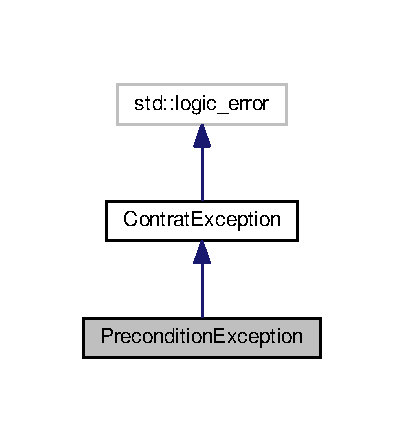
\includegraphics[width=194pt]{classPreconditionException__inherit__graph}
\end{center}
\end{figure}


Collaboration diagram for Precondition\+Exception\+:\nopagebreak
\begin{figure}[H]
\begin{center}
\leavevmode
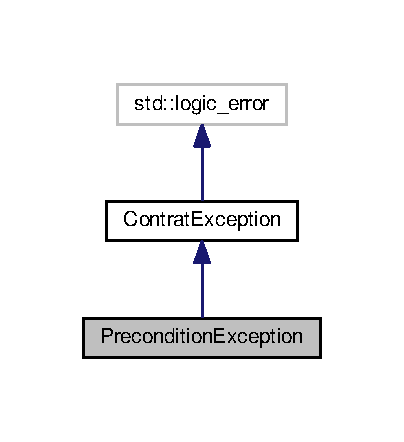
\includegraphics[width=194pt]{classPreconditionException__coll__graph}
\end{center}
\end{figure}
\subsection*{Public Member Functions}
\begin{DoxyCompactItemize}
\item 
\hyperlink{classPreconditionException_a66d4b4c57a0675d487dab85d2c31b08c}{Precondition\+Exception} (std\+::string, unsigned int, std\+::string)
\begin{DoxyCompactList}\small\item\em Constructeur de la classe \hyperlink{classPreconditionException}{Precondition\+Exception} en initialisant la classe de base \hyperlink{classContratException}{Contrat\+Exception}. La classe représente l\textquotesingle{}erreur de précondition dans la théorie du contrat. \end{DoxyCompactList}\end{DoxyCompactItemize}


\subsection{Constructor \& Destructor Documentation}
\hypertarget{classPreconditionException_a66d4b4c57a0675d487dab85d2c31b08c}{}\index{Precondition\+Exception@{Precondition\+Exception}!Precondition\+Exception@{Precondition\+Exception}}
\index{Precondition\+Exception@{Precondition\+Exception}!Precondition\+Exception@{Precondition\+Exception}}
\subsubsection[{Precondition\+Exception}]{\setlength{\rightskip}{0pt plus 5cm}Precondition\+Exception\+::\+Precondition\+Exception (
\begin{DoxyParamCaption}
\item[{std\+::string}]{p\+\_\+fich\+P, }
\item[{unsigned int}]{p\+\_\+prm\+Ligne, }
\item[{std\+::string}]{p\+\_\+expr\+P}
\end{DoxyParamCaption}
)}\label{classPreconditionException_a66d4b4c57a0675d487dab85d2c31b08c}


Constructeur de la classe \hyperlink{classPreconditionException}{Precondition\+Exception} en initialisant la classe de base \hyperlink{classContratException}{Contrat\+Exception}. La classe représente l\textquotesingle{}erreur de précondition dans la théorie du contrat. 


\begin{DoxyParams}{Parameters}
{\em p\+\_\+fich\+P} & chaîne de caractères représentant le fichier source dans lequel a eu lieu l\textquotesingle{}erreur \\
\hline
{\em p\+\_\+prm\+Ligne} & un entier représentant la ligne où a eu lieu l\textquotesingle{}erreur \\
\hline
{\em p\+\_\+expr\+P} & Test logique qui a échoué \\
\hline
\end{DoxyParams}


The documentation for this class was generated from the following files\+:\begin{DoxyCompactItemize}
\item 
\hyperlink{ContratException_8h}{Contrat\+Exception.\+h}\item 
\hyperlink{ContratException_8cpp}{Contrat\+Exception.\+cpp}\end{DoxyCompactItemize}

\hypertarget{classtp_1_1Reference}{}\section{tp\+:\+:Reference Class Reference}
\label{classtp_1_1Reference}\index{tp\+::\+Reference@{tp\+::\+Reference}}


Classe permettant de documenter une reference.  




{\ttfamily \#include $<$Reference.\+h$>$}



Inheritance diagram for tp\+:\+:Reference\+:\nopagebreak
\begin{figure}[H]
\begin{center}
\leavevmode
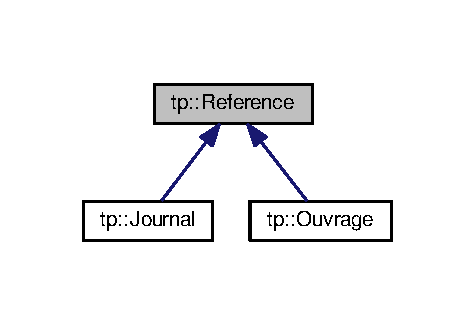
\includegraphics[width=228pt]{classtp_1_1Reference__inherit__graph}
\end{center}
\end{figure}
\subsection*{Public Member Functions}
\begin{DoxyCompactItemize}
\item 
\hyperlink{classtp_1_1Reference_acea8bdd14988b8b699bc0fb78bca6302}{Reference} (const std\+::string \&p\+\_\+auteurs=\char`\"{}Paul Chevalier\char`\"{}, const std\+::string \&p\+\_\+titre=\char`\"{}Speed Kills\char`\"{}, const std\+::string \&p\+\_\+identifiant=\char`\"{}978332256430\char`\"{}, unsigned p\+\_\+annee=2014)
\begin{DoxyCompactList}\small\item\em Constructeur de la classe \hyperlink{classtp_1_1Reference}{Reference} Les parametres de cette classe sont\+: \end{DoxyCompactList}\item 
const std\+::string \& \hyperlink{classtp_1_1Reference_abfdff53e68702977fb384a50b01c0f00}{req\+Auteurs} () const 
\item 
const std\+::string \& \hyperlink{classtp_1_1Reference_ae08e4a53bf172bb0bd208150a5c5699d}{req\+Titre} () const 
\item 
const std\+::string \& \hyperlink{classtp_1_1Reference_adfad13c3fb4a9e0eae59e0945c66666e}{req\+Identifiant} () const 
\item 
unsigned \hyperlink{classtp_1_1Reference_ace181178a68541f6794f8fb4f69d2aee}{req\+Annee} () const 
\item 
\hypertarget{classtp_1_1Reference_a5f2610f7f46ec237f69a73f2ba58ba78}{}void \hyperlink{classtp_1_1Reference_a5f2610f7f46ec237f69a73f2ba58ba78}{asg\+Auteurs} (const std\+::string \&p\+\_\+auteurs)\label{classtp_1_1Reference_a5f2610f7f46ec237f69a73f2ba58ba78}

\begin{DoxyCompactList}\small\item\em Mutateur pour auteurs, modifie les auteurs. \end{DoxyCompactList}\item 
\hypertarget{classtp_1_1Reference_a42ae9fbbfdbe64d1fb2b6b4eb2a6466a}{}void \hyperlink{classtp_1_1Reference_a42ae9fbbfdbe64d1fb2b6b4eb2a6466a}{asg\+Titre} (const std\+::string \&p\+\_\+titre)\label{classtp_1_1Reference_a42ae9fbbfdbe64d1fb2b6b4eb2a6466a}

\begin{DoxyCompactList}\small\item\em Mutateur pour titre, modifie le titre. \end{DoxyCompactList}\item 
\hypertarget{classtp_1_1Reference_aa1a84679155a34d39b3f115ffb779257}{}void \hyperlink{classtp_1_1Reference_aa1a84679155a34d39b3f115ffb779257}{asg\+Identifiant} (const std\+::string \&p\+\_\+identifiant)\label{classtp_1_1Reference_aa1a84679155a34d39b3f115ffb779257}

\begin{DoxyCompactList}\small\item\em Mutateur pour identifiant, modifie l\textquotesingle{}identifiant. \end{DoxyCompactList}\item 
\hypertarget{classtp_1_1Reference_ab793e0c7d61b5972c2937152722f48cb}{}void \hyperlink{classtp_1_1Reference_ab793e0c7d61b5972c2937152722f48cb}{asg\+Annee} (unsigned p\+\_\+annee)\label{classtp_1_1Reference_ab793e0c7d61b5972c2937152722f48cb}

\begin{DoxyCompactList}\small\item\em Mutateur pour annee, modifie l\textquotesingle{}annee. \end{DoxyCompactList}\item 
\hypertarget{classtp_1_1Reference_ac2fc9e39760fb00287556c3fa6fed386}{}bool {\bfseries operator==} (const \hyperlink{classtp_1_1Reference}{Reference} \&p\+\_\+reference)\label{classtp_1_1Reference_ac2fc9e39760fb00287556c3fa6fed386}

\item 
virtual std\+::string \hyperlink{classtp_1_1Reference_af166101d908f6d0f8edeb8624aa77a9b}{req\+Reference\+Formate} () const =0
\item 
\hypertarget{classtp_1_1Reference_a01028cf0d5f94314ce00e38ccad96089}{}virtual \hyperlink{classtp_1_1Reference}{Reference} $\ast$ {\bfseries clone} () const =0\label{classtp_1_1Reference_a01028cf0d5f94314ce00e38ccad96089}

\end{DoxyCompactItemize}


\subsection{Detailed Description}
Classe permettant de documenter une reference. 

de la classe de base \hyperlink{classtp_1_1Reference}{Reference} 

\subsection{Constructor \& Destructor Documentation}
\hypertarget{classtp_1_1Reference_acea8bdd14988b8b699bc0fb78bca6302}{}\index{tp\+::\+Reference@{tp\+::\+Reference}!Reference@{Reference}}
\index{Reference@{Reference}!tp\+::\+Reference@{tp\+::\+Reference}}
\subsubsection[{Reference}]{\setlength{\rightskip}{0pt plus 5cm}tp\+::\+Reference\+::\+Reference (
\begin{DoxyParamCaption}
\item[{const std\+::string \&}]{p\+\_\+auteurs = {\ttfamily \char`\"{}Paul~Chevalier\char`\"{}}, }
\item[{const std\+::string \&}]{p\+\_\+titre = {\ttfamily \char`\"{}Speed~Kills\char`\"{}}, }
\item[{const std\+::string \&}]{p\+\_\+identifiant = {\ttfamily \char`\"{}978332256430\char`\"{}}, }
\item[{unsigned}]{p\+\_\+annee = {\ttfamily 2014}}
\end{DoxyParamCaption}
)}\label{classtp_1_1Reference_acea8bdd14988b8b699bc0fb78bca6302}


Constructeur de la classe \hyperlink{classtp_1_1Reference}{Reference} Les parametres de cette classe sont\+: 


\begin{DoxyParams}{Parameters}
{\em p\+\_\+auteurs} & du référence \\
\hline
{\em p\+\_\+titre} & du référence \\
\hline
{\em p\+\_\+identifiant} & du référence \\
\hline
{\em p\+\_\+annee} & du référence \\
\hline
{\em p\+\_\+ville} & du référence \\
\hline
{\em p\+\_\+editeur} & du référence \\
\hline
\end{DoxyParams}


\subsection{Member Function Documentation}
\hypertarget{classtp_1_1Reference_ace181178a68541f6794f8fb4f69d2aee}{}\index{tp\+::\+Reference@{tp\+::\+Reference}!req\+Annee@{req\+Annee}}
\index{req\+Annee@{req\+Annee}!tp\+::\+Reference@{tp\+::\+Reference}}
\subsubsection[{req\+Annee}]{\setlength{\rightskip}{0pt plus 5cm}unsigned tp\+::\+Reference\+::req\+Annee (
\begin{DoxyParamCaption}
{}
\end{DoxyParamCaption}
) const}\label{classtp_1_1Reference_ace181178a68541f6794f8fb4f69d2aee}
brief Acceseur pour req\+Annee return m\+\_\+annee l\textquotesingle{}annee de l\textquotesingle{}objet \hypertarget{classtp_1_1Reference_abfdff53e68702977fb384a50b01c0f00}{}\index{tp\+::\+Reference@{tp\+::\+Reference}!req\+Auteurs@{req\+Auteurs}}
\index{req\+Auteurs@{req\+Auteurs}!tp\+::\+Reference@{tp\+::\+Reference}}
\subsubsection[{req\+Auteurs}]{\setlength{\rightskip}{0pt plus 5cm}const std\+::string \& tp\+::\+Reference\+::req\+Auteurs (
\begin{DoxyParamCaption}
{}
\end{DoxyParamCaption}
) const}\label{classtp_1_1Reference_abfdff53e68702977fb384a50b01c0f00}
brief Acceseur pour req\+Auteur return m\+\_\+auteur l\textquotesingle{}auteur de l\textquotesingle{}objet \hypertarget{classtp_1_1Reference_adfad13c3fb4a9e0eae59e0945c66666e}{}\index{tp\+::\+Reference@{tp\+::\+Reference}!req\+Identifiant@{req\+Identifiant}}
\index{req\+Identifiant@{req\+Identifiant}!tp\+::\+Reference@{tp\+::\+Reference}}
\subsubsection[{req\+Identifiant}]{\setlength{\rightskip}{0pt plus 5cm}const std\+::string \& tp\+::\+Reference\+::req\+Identifiant (
\begin{DoxyParamCaption}
{}
\end{DoxyParamCaption}
) const}\label{classtp_1_1Reference_adfad13c3fb4a9e0eae59e0945c66666e}
brief Acceseur pour req\+Identifiant return m\+\_\+identifiant l\textquotesingle{}identiiant de l\textquotesingle{}objet \hypertarget{classtp_1_1Reference_af166101d908f6d0f8edeb8624aa77a9b}{}\index{tp\+::\+Reference@{tp\+::\+Reference}!req\+Reference\+Formate@{req\+Reference\+Formate}}
\index{req\+Reference\+Formate@{req\+Reference\+Formate}!tp\+::\+Reference@{tp\+::\+Reference}}
\subsubsection[{req\+Reference\+Formate}]{\setlength{\rightskip}{0pt plus 5cm}std\+::string tp\+::\+Reference\+::req\+Reference\+Formate (
\begin{DoxyParamCaption}
{}
\end{DoxyParamCaption}
) const\hspace{0.3cm}{\ttfamily [pure virtual]}}\label{classtp_1_1Reference_af166101d908f6d0f8edeb8624aa77a9b}
brief Acceseur pour pour req\+Reference\+Formate return le format des références 

Implemented in \hyperlink{classtp_1_1Journal_adbc714005b9d394b6b76ba7f5f9f560f}{tp\+::\+Journal}, and \hyperlink{classtp_1_1Ouvrage_a72a27ae3d11d41e3f02021c671e9a50a}{tp\+::\+Ouvrage}.

\hypertarget{classtp_1_1Reference_ae08e4a53bf172bb0bd208150a5c5699d}{}\index{tp\+::\+Reference@{tp\+::\+Reference}!req\+Titre@{req\+Titre}}
\index{req\+Titre@{req\+Titre}!tp\+::\+Reference@{tp\+::\+Reference}}
\subsubsection[{req\+Titre}]{\setlength{\rightskip}{0pt plus 5cm}const std\+::string \& tp\+::\+Reference\+::req\+Titre (
\begin{DoxyParamCaption}
{}
\end{DoxyParamCaption}
) const}\label{classtp_1_1Reference_ae08e4a53bf172bb0bd208150a5c5699d}
brief Acceseur pour req\+Titre return m\+\_\+titre le titre de l\textquotesingle{}objet 

The documentation for this class was generated from the following files\+:\begin{DoxyCompactItemize}
\item 
Reference.\+h\item 
Reference.\+cpp\end{DoxyCompactItemize}

\hypertarget{classtp_1_1ReferenceAbsenteException}{}\section{tp\+:\+:Reference\+Absente\+Exception Class Reference}
\label{classtp_1_1ReferenceAbsenteException}\index{tp\+::\+Reference\+Absente\+Exception@{tp\+::\+Reference\+Absente\+Exception}}


Inheritance diagram for tp\+:\+:Reference\+Absente\+Exception\+:\nopagebreak
\begin{figure}[H]
\begin{center}
\leavevmode
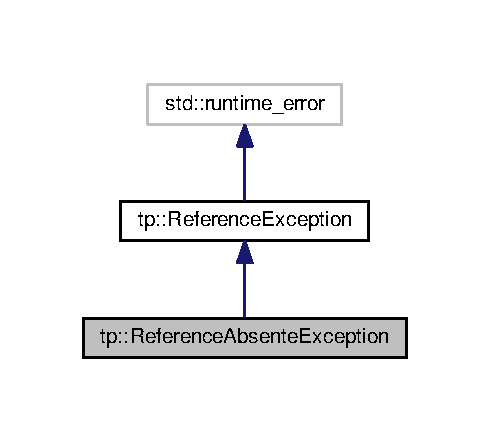
\includegraphics[width=235pt]{classtp_1_1ReferenceAbsenteException__inherit__graph}
\end{center}
\end{figure}


Collaboration diagram for tp\+:\+:Reference\+Absente\+Exception\+:\nopagebreak
\begin{figure}[H]
\begin{center}
\leavevmode
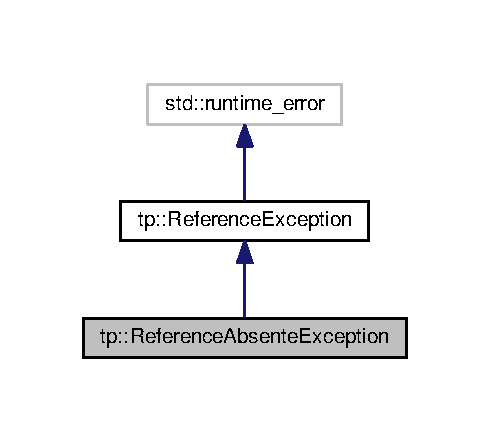
\includegraphics[width=235pt]{classtp_1_1ReferenceAbsenteException__coll__graph}
\end{center}
\end{figure}
\subsection*{Public Member Functions}
\begin{DoxyCompactItemize}
\item 
\hypertarget{classtp_1_1ReferenceAbsenteException_a87407d5bb43f9563a8b0f7322b15ad13}{}{\bfseries Reference\+Absente\+Exception} (const std\+::string \&p\+\_\+raison)\label{classtp_1_1ReferenceAbsenteException_a87407d5bb43f9563a8b0f7322b15ad13}

\end{DoxyCompactItemize}


The documentation for this class was generated from the following files\+:\begin{DoxyCompactItemize}
\item 
Reference\+Absente\+Exception.\+h\item 
Reference\+Absente\+Exception.\+cpp\end{DoxyCompactItemize}

\hypertarget{classtp_1_1ReferenceDejaPresenteException}{}\section{tp\+:\+:Reference\+Deja\+Presente\+Exception Class Reference}
\label{classtp_1_1ReferenceDejaPresenteException}\index{tp\+::\+Reference\+Deja\+Presente\+Exception@{tp\+::\+Reference\+Deja\+Presente\+Exception}}


Inheritance diagram for tp\+:\+:Reference\+Deja\+Presente\+Exception\+:\nopagebreak
\begin{figure}[H]
\begin{center}
\leavevmode
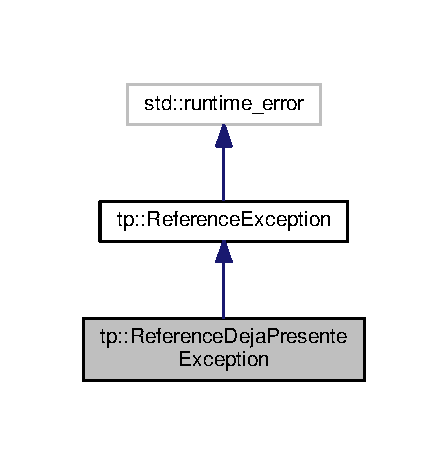
\includegraphics[width=215pt]{classtp_1_1ReferenceDejaPresenteException__inherit__graph}
\end{center}
\end{figure}


Collaboration diagram for tp\+:\+:Reference\+Deja\+Presente\+Exception\+:\nopagebreak
\begin{figure}[H]
\begin{center}
\leavevmode
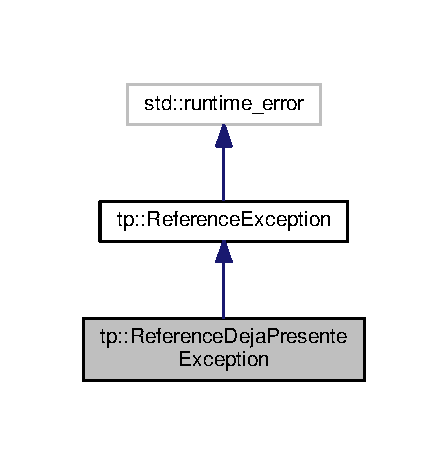
\includegraphics[width=215pt]{classtp_1_1ReferenceDejaPresenteException__coll__graph}
\end{center}
\end{figure}
\subsection*{Public Member Functions}
\begin{DoxyCompactItemize}
\item 
\hypertarget{classtp_1_1ReferenceDejaPresenteException_af9f1bc5c47b3519182bdbdf4bc84e247}{}{\bfseries Reference\+Deja\+Presente\+Exception} (const std\+::string \&p\+\_\+raison)\label{classtp_1_1ReferenceDejaPresenteException_af9f1bc5c47b3519182bdbdf4bc84e247}

\end{DoxyCompactItemize}


The documentation for this class was generated from the following files\+:\begin{DoxyCompactItemize}
\item 
Reference\+Deja\+Presente\+Exception.\+h\item 
Reference\+Deja\+Presente\+Exception.\+cpp\end{DoxyCompactItemize}

\hypertarget{classtp_1_1ReferenceException}{}\section{tp\+:\+:Reference\+Exception Class Reference}
\label{classtp_1_1ReferenceException}\index{tp\+::\+Reference\+Exception@{tp\+::\+Reference\+Exception}}


Inheritance diagram for tp\+:\+:Reference\+Exception\+:\nopagebreak
\begin{figure}[H]
\begin{center}
\leavevmode
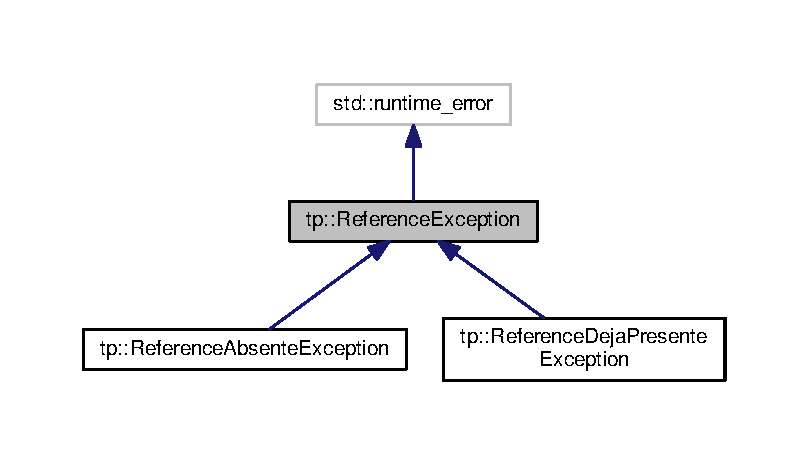
\includegraphics[width=350pt]{classtp_1_1ReferenceException__inherit__graph}
\end{center}
\end{figure}


Collaboration diagram for tp\+:\+:Reference\+Exception\+:\nopagebreak
\begin{figure}[H]
\begin{center}
\leavevmode
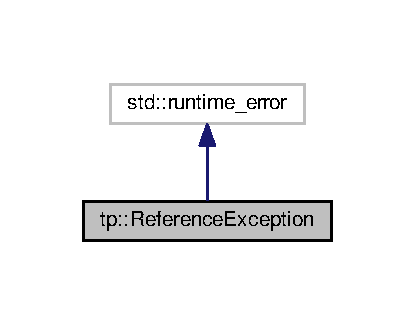
\includegraphics[width=199pt]{classtp_1_1ReferenceException__coll__graph}
\end{center}
\end{figure}
\subsection*{Public Member Functions}
\begin{DoxyCompactItemize}
\item 
\hypertarget{classtp_1_1ReferenceException_ac3553090925711e06bdad4d1cd38c78e}{}{\bfseries Reference\+Exception} (const std\+::string \&p\+\_\+raison)\label{classtp_1_1ReferenceException_ac3553090925711e06bdad4d1cd38c78e}

\end{DoxyCompactItemize}


The documentation for this class was generated from the following files\+:\begin{DoxyCompactItemize}
\item 
Reference\+Exception.\+h\item 
Reference\+Exception.\+cpp\end{DoxyCompactItemize}

\chapter{File Documentation}
\hypertarget{ContratException_8cpp}{}\section{Contrat\+Exception.\+cpp File Reference}
\label{ContratException_8cpp}\index{Contrat\+Exception.\+cpp@{Contrat\+Exception.\+cpp}}


Implantation de la classe \hyperlink{classContratException}{Contrat\+Exception} et de ses héritiers.  


{\ttfamily \#include \char`\"{}Contrat\+Exception.\+h\char`\"{}}\\*
{\ttfamily \#include $<$sstream$>$}\\*
Include dependency graph for Contrat\+Exception.\+cpp\+:\nopagebreak
\begin{figure}[H]
\begin{center}
\leavevmode
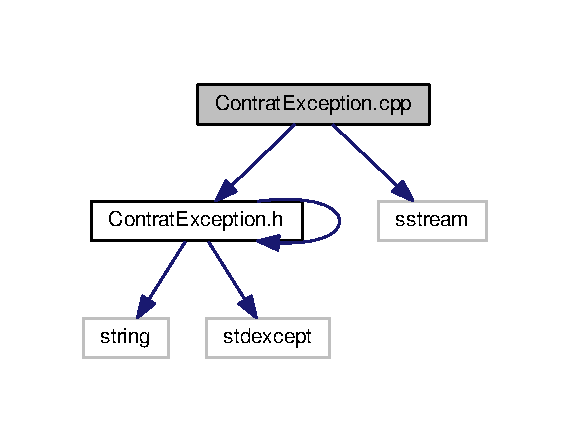
\includegraphics[width=273pt]{ContratException_8cpp__incl}
\end{center}
\end{figure}


\subsection{Detailed Description}
Implantation de la classe \hyperlink{classContratException}{Contrat\+Exception} et de ses héritiers. 

\begin{DoxyAuthor}{Author}
administrateur 
\end{DoxyAuthor}
\begin{DoxyDate}{Date}
16 janvier 2014 
\end{DoxyDate}
\begin{DoxyVersion}{Version}
révisée balises Doxygen C++ normes H2014 
\end{DoxyVersion}

\hypertarget{ContratException_8h}{}\section{Contrat\+Exception.\+h File Reference}
\label{ContratException_8h}\index{Contrat\+Exception.\+h@{Contrat\+Exception.\+h}}


D�claration de la classe \hyperlink{classContratException}{Contrat\+Exception} et de ses h�ritiers\+: std\+::logic\+\_\+error Classe de base des exceptions logiques \hyperlink{classContratException}{Contrat\+Exception}\+: Classe de base des exceptions de contrat. \hyperlink{classAssertionException}{Assertion\+Exception}\+: Classe de gestion des erreurs d\textquotesingle{}assertion. \hyperlink{classPreconditionException}{Precondition\+Exception}\+: Classe de gestion des erreurs de pr�condition. \hyperlink{classPostconditionException}{Postcondition\+Exception}\+: Classe de gestion des erreurs de postcondition. \hyperlink{classInvariantException}{Invariant\+Exception}\+: Classe de gestion des erreurs d\textquotesingle{}invariant.  


{\ttfamily \#include \char`\"{}Contrat\+Exception.\+h\char`\"{}}\\*
{\ttfamily \#include $<$string$>$}\\*
{\ttfamily \#include $<$stdexcept$>$}\\*
Include dependency graph for Contrat\+Exception.\+h\+:\nopagebreak
\begin{figure}[H]
\begin{center}
\leavevmode
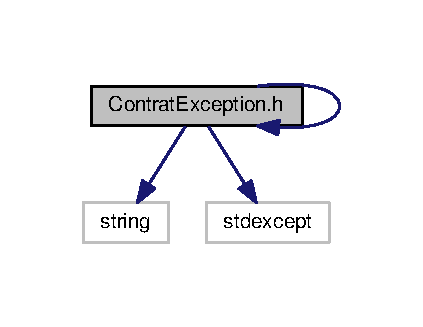
\includegraphics[width=203pt]{ContratException_8h__incl}
\end{center}
\end{figure}
This graph shows which files directly or indirectly include this file\+:\nopagebreak
\begin{figure}[H]
\begin{center}
\leavevmode
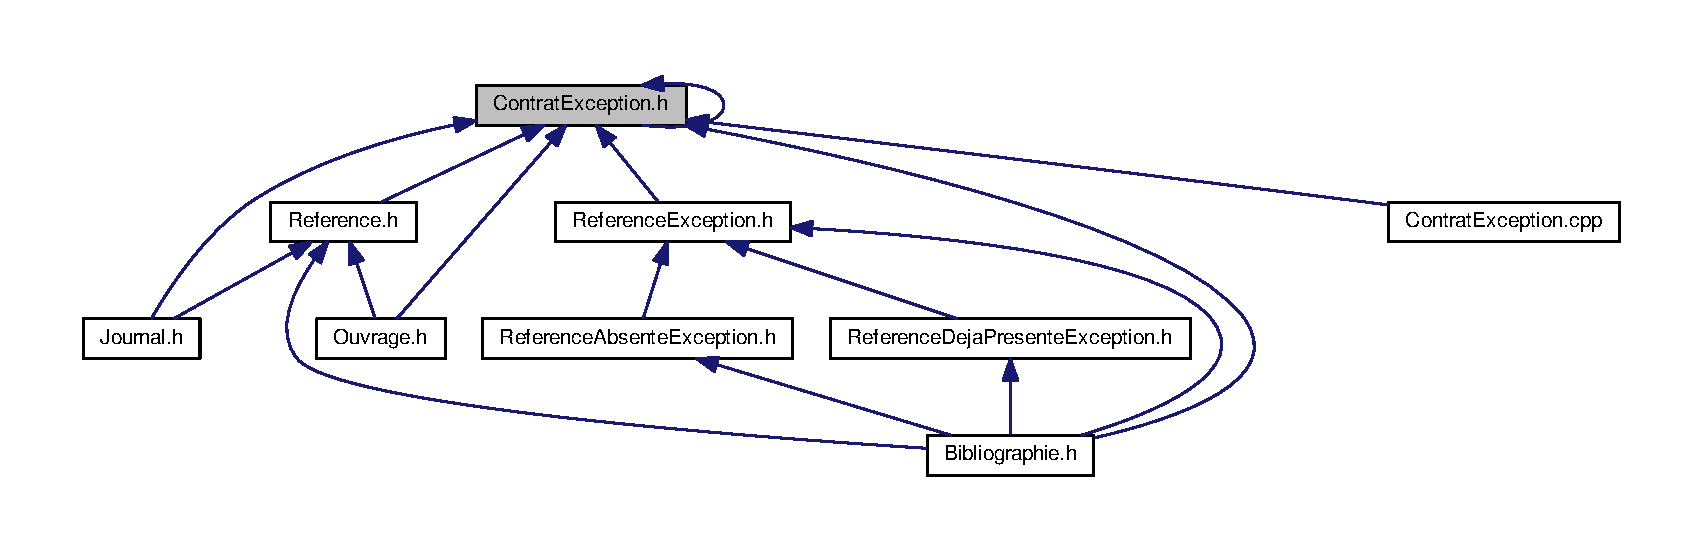
\includegraphics[width=350pt]{ContratException_8h__dep__incl}
\end{center}
\end{figure}
\subsection*{Classes}
\begin{DoxyCompactItemize}
\item 
class \hyperlink{classContratException}{Contrat\+Exception}
\item 
class \hyperlink{classAssertionException}{Assertion\+Exception}
\item 
class \hyperlink{classPreconditionException}{Precondition\+Exception}
\item 
class \hyperlink{classPostconditionException}{Postcondition\+Exception}
\item 
class \hyperlink{classInvariantException}{Invariant\+Exception}
\end{DoxyCompactItemize}
\subsection*{Macros}
\begin{DoxyCompactItemize}
\item 
\hypertarget{ContratException_8h_a52dddc2c198c58b53b201c313934e40c}{}\#define {\bfseries I\+N\+V\+A\+R\+I\+A\+N\+T\+S}()~verifie\+Invariant()\label{ContratException_8h_a52dddc2c198c58b53b201c313934e40c}

\item 
\hypertarget{ContratException_8h_abe6e3e0ff48f8595570e6485b506a8c4}{}\#define {\bfseries A\+S\+S\+E\+R\+T\+I\+O\+N}(f)~if (!(f)) throw \hyperlink{classAssertionException}{Assertion\+Exception}(\+\_\+\+\_\+\+F\+I\+L\+E\+\_\+\+\_\+,\+\_\+\+\_\+\+L\+I\+N\+E\+\_\+\+\_\+, \#f);\label{ContratException_8h_abe6e3e0ff48f8595570e6485b506a8c4}

\item 
\hypertarget{ContratException_8h_acb3361bd87fc697a57b7286a9998c106}{}\#define {\bfseries P\+R\+E\+C\+O\+N\+D\+I\+T\+I\+O\+N}(f)~if (!(f)) throw \hyperlink{classPreconditionException}{Precondition\+Exception}(\+\_\+\+\_\+\+F\+I\+L\+E\+\_\+\+\_\+, \+\_\+\+\_\+\+L\+I\+N\+E\+\_\+\+\_\+, \#f);\label{ContratException_8h_acb3361bd87fc697a57b7286a9998c106}

\item 
\hypertarget{ContratException_8h_a438b75c0c77a1ce8d1e914f9f04ea548}{}\#define {\bfseries P\+O\+S\+T\+C\+O\+N\+D\+I\+T\+I\+O\+N}(f)~if (!(f)) throw \hyperlink{classPostconditionException}{Postcondition\+Exception}(\+\_\+\+\_\+\+F\+I\+L\+E\+\_\+\+\_\+, \+\_\+\+\_\+\+L\+I\+N\+E\+\_\+\+\_\+, \#f);\label{ContratException_8h_a438b75c0c77a1ce8d1e914f9f04ea548}

\item 
\hypertarget{ContratException_8h_a08f80155f47e05681c2b9bb9c5f6fffe}{}\#define {\bfseries I\+N\+V\+A\+R\+I\+A\+N\+T}(f)~if (!(f)) throw \hyperlink{classInvariantException}{Invariant\+Exception}(\+\_\+\+\_\+\+F\+I\+L\+E\+\_\+\+\_\+,\+\_\+\+\_\+\+L\+I\+N\+E\+\_\+\+\_\+, \#f);\label{ContratException_8h_a08f80155f47e05681c2b9bb9c5f6fffe}

\end{DoxyCompactItemize}


\subsection{Detailed Description}
D�claration de la classe \hyperlink{classContratException}{Contrat\+Exception} et de ses h�ritiers\+: std\+::logic\+\_\+error Classe de base des exceptions logiques \hyperlink{classContratException}{Contrat\+Exception}\+: Classe de base des exceptions de contrat. \hyperlink{classAssertionException}{Assertion\+Exception}\+: Classe de gestion des erreurs d\textquotesingle{}assertion. \hyperlink{classPreconditionException}{Precondition\+Exception}\+: Classe de gestion des erreurs de pr�condition. \hyperlink{classPostconditionException}{Postcondition\+Exception}\+: Classe de gestion des erreurs de postcondition. \hyperlink{classInvariantException}{Invariant\+Exception}\+: Classe de gestion des erreurs d\textquotesingle{}invariant. 

\begin{DoxyAuthor}{Author}
administrateur 
\end{DoxyAuthor}
\begin{DoxyDate}{Date}
16 juin 2011 
\end{DoxyDate}
\begin{DoxyVersion}{Version}
r�vis�e 14 f�vrier 2012 balises Doxygen C++ 
\end{DoxyVersion}

%--- End generated contents ---

% Index
\backmatter
\newpage
\phantomsection
\clearemptydoublepage
\addcontentsline{toc}{chapter}{Index}
\printindex

\end{document}
